\chapter{Algoritmer} \label{kap.algo}
Dette kapitel tager udgangspunkt i \citep{dmat}.

Når man står med et problem inden for diskret matematik, er det første, man skal gøre at finde en model, der kan sætte problemet i matematisk kontekst. Denne model skal bestå af diskrete strukturer såsom tællelige følger eller grafer. Når man har opstillet en passende model til at løse problemet, skal man finde en metode, som kan løse det med denne model. Denne metode skal helst tilpasses, så den kan løse det generelle problem, det vil sige alle probemer af den type og form. Et eksempel på en sådan metode er en \emph{algoritme}.
\begin{defn}
[Algoritmer] En algoritme er en begrænset mængde af præcist definerede instruktioner, der viser, hvordan et problem løses, eller hvordan en beregning udføres. 
\end{defn}

Der er nogle kendetegn, man ønsker skal gøre sig gældende for den algoritme, man anvender til at løse sit problem. Herunder, at den giver et korrekt output til et givent input. Det er derudover lettere at arbejde med algoritmer, som er \emph{begrænsede}, og dermed ikke har uendeligt mange trin. Algoritmen bør være effektiv, så man præcist og indenfor et begrænset tidsrum kan løse problemet. Slutteligt bør algoritmen være generel, så den er anvendelig på alle problemer af denne type og form.

I følgende afsnit vil vi skrive alle algoritmer i pseudokode, som er en forsimplet form for programmeringssprog. Pseudokode kan ikke direkte implementeres i nogen programmer, da det ikke har en bestemt syntaks. Grunden til, at vi skriver algoritmerne i pseudokode, er, at det er nemt at omskrive til forskellige andre programmeringssprog.


\section{Algoritmetyper}
Der findes mange typer algoritmer, som løser mange forskellige problemer. Vi vil i det følgende se på forskellige typer af algoritmer.
\subsection{Søgealgoritmer}
\emph{Søgealgoritmer} bruges til at løse problemer, hvor man vil finde et element, $x$, i en liste $(a_{1}, a_{2}, \dotsc, a_{n})$, eller konkludere, at $x$ ikke er i listen. Her vil løsningen være $i$, hvis $x=a_{i}$. Det er altså indekset, der er løsningen. Søgealgoritmer kan igen opdeles i forskellige typer bl.a. \emph{den lineære søgning} og \emph{den binære søgning}. Ved den lineære søgning starter man med $a_1$ og ser, om $x=a_{1}$. Hvis dette er tilfældet, er $a_{1}$'s indeks svaret, men hvis $x \neq a_{1}$, fortsætter man til $a_{2}$ og så $a_{3}$. Sådan fortsætter man, indtil man finder et element i listen, der er lig $x$, og så vil løsningen være dette elements indeks. \autoref{alg:lineaer} illustrerer et eksempel på en lineær søgealgoritme:

\begin{algorithm}[H] 
\caption{Den lineære søgealgoritme}
\begin{algorithmic}[1]

\Procedure{lineær søgning($x$: heltal, $a_{1},a_{2},\dotsc,a_{n}$: Heltal i listen)}{}
    \State $i:=1$
    \While{$i \leq n$ \textbf{and} $x \neq a_{i}$}
        \State $i:=i+1$
    \EndWhile
    \If{$i \leq n$} 
    \State \textbf{return} $lokation:=i$
    \Else
    \State \textbf{return} $lokation:=0$
    \EndIf
  \label{roy's loop}
\EndProcedure

\end{algorithmic}
\label{alg:lineaer}
\end{algorithm}


Modsat den lineære søgning kan den binære søgning kun bruges, når en liste er \emph{ordnet}. Det vil sige, hvis listen fx er voksende, aftagende eller alfabetisk, altså $(a_{1}<a_{2}<\dotsb<a_{n})$. Den binære søgealgoritme finder nu midten af listen, $a_{m}$, hvor $m=\left \lfloor \frac{n+1}{2} \right \rfloor$. $\lfloor \rfloor$ er flooroperatoren der runder ned til første heltal. Vi ser nu, hvilken side det, vi søger, er på. Hvis $a_{m}<x$, tager vi halvdelen af listen, der er større end $a_{m}$ dvs: $(a_{m+1}, a_{m+2},\dotsc,a_{n})$. Ellers tager vi halvdelen mindre end og lig $a_{m}$: $(a_{1}, a_{2},\dotsc,a_{m})$. Når vi har vurderet hvilken side af midten, den værdi, vi søger, er på, deles denne halvdel på midten, hvorefter man igen skal vurdere, hvilken side man skal arbejde videre med. Dette fortsættes, indtil tallet er fundet. Den binære søgealgoritme er illustreret i \autoref{alg:binaer}.

\begin{algorithm}[H]
\caption{Den binære søgealgoritme}
\begin{algorithmic}[1]

\Procedure{binær søgning($x$: heltal, $a_{1},a_{2},\dotsc,a_{n}$: Voksende heltal i listen)}{}
    \State $i:=1$, \{$i$ er venstre endepunkt i søgeintervallet\}
    \State $j:=n$, \{$j$ er højre endepunkt i søgeintervallet\}
    \While{$i<j$}
        \State $m=\lfloor (i+j)/2 \rfloor$
    		\If{$x>a_{m}$}
    		\State $i:=m+1$
    		\Else
    		\State $j:=m$
    		\EndIf    
    \EndWhile
    \If {$x=a_{i}$}
    	\State \textbf{return} $lokation:=i$
    \Else
    	\State \textbf{return} $lokation:=0$
    \EndIf
  \label{roy's loop}
\EndProcedure

\end{algorithmic}
\label{alg:binaer}
\end{algorithm}

\subsection{Sorteringsalgoritmer} \label{kap:sortering}
Når vi arbejder med \emph{sorteringsalgoritmer}, er det, fordi vi ønsker at sortere en liste, således at den inddeles i fx voksende rækkefølge eller alfabetisk orden. Ligesom ved søgealgoritmerne er der flere forskellige sorteringsalgoritmer. Eksempler på disse er \emph{bubblesortering} og \emph{indskudssortering}. Bubblesortering er en af de simpleste sorteringsalgoritmer, men den er ikke så effektiv. Vi vil komme ind på algoritmers effektivitet i \autoref{kap:kompleksitet}. Den sammenligner tilstødende værdier i en liste og bytter om på dem, hvis rækkefølgen ikke er korrekt.

\begin{algorithm}[H]
\caption{Bubblesorteringsalgoritmen}
\begin{algorithmic}[1]

\Procedure{bubblesortering($a_{1},a_{2},\dotsc,a_{n}$: Reelle tal hvor $n \geq 2$)}{}
\EndProcedure
\For {$i:=1$ \textbf{to} $n-1$}
    	\For {$j:=1$ \textbf{to} $n-i$}
    		\If {$a_{j}>a_{j+1}$}
    			\State Ombyt $a_{j}$ og $a_{j+1}$ 	
\EndIf
\EndFor
\EndFor
\State $a_{1},a_{2},\dotsc,a_{n}$ er i voksende rækkefølge. 

\end{algorithmic}
\end{algorithm}

\begin{exmp}
Vi ser på en liste, $(3,4,2,5,1)$, som vi vil arrangere således, at den er i rækkefølge med stigende værdi. Algoritmen gentages fire gange, da listen har længden $n=5$, og algoritmen skal køre $n-1$ gange. 
\begin{align*}
	\text{Første gentagelse:} \qquad \qquad \qquad \quad \text{Anden 			gentagelse:} \qquad \qquad \qquad \quad \text{Tredje gentagelse:} 			\qquad \qquad \qquad \quad \\
	(\textbf{3,4},2,5,1) \rightarrow (\textbf{3,4},2,5,1) \qquad \qquad 		(\textbf{3,2},4,1,5) \rightarrow (\textbf{2,3},4,1,5) \qquad \qquad 		(\textbf{2,3},1,4,5) \rightarrow (\textbf{2,3},1,4,5) \qquad \qquad 		\\
	(3,\textbf{4,2},5,1) \rightarrow (3,\textbf{2,4},5,1) \qquad \qquad     	(2,\textbf{3,1},4,5) \rightarrow (2,\textbf{1,3},4,5) \qquad \qquad   	(2,\textbf{3,1},4,5) \rightarrow (2,\textbf{1,3},4,5) \qquad \qquad 		\\
	(3,2,\textbf{4,5},1) \rightarrow (3,2,\textbf{4,5},1) \qquad \qquad 		(2,1,\textbf{3,4},5) \rightarrow (2,1,\textbf{3,4},5) \qquad \qquad  	\qquad \qquad \qquad \qquad \qquad \qquad \qquad \quad \ \ \\
	(3,2,4,\textbf{5,1}) \rightarrow (3,2,4,\textbf{1,5}) \qquad \qquad 		\qquad \qquad \qquad \qquad \qquad \qquad \qquad \quad \ \  \qquad 			\qquad \qquad \qquad \qquad \qquad \qquad \quad \ \
\end{align*}

\begin{flushleft}
Fjerde gentagelse:
\\
$(\textbf{2,1},3,4,5) \rightarrow (\textbf{1,2},3,4,5)$
\end{flushleft}

Efter første gentagelse har algoitmen placeres det største tal bagerst i listen, efter anden gentagelse har algoritmen placeret det næst største tal på næst sidste plads i listen. Således fortsætter algoritmen indtil listen er i korrekt rækkefølge.

\end{exmp}

Indskudssortering er på samme måde som bubblesortering simpel og til tider ineffektiv. For denne algoritme gælder det, at man starter med den anden værdi i listen, som sammenlignes med den første værdi. Disse to sorteres nu efter størrelse. Den tredje værdi i listen sammenlignes derefter med den første. Hvis den er større, sammenlignes den med den anden værdi i listen, og på den måde sorteres hele rækken, så de til sidst står i rækkefølge.

\begin{algorithm}[H]
\caption{Indskudssorteringsalgoritmen}
\begin{algorithmic}[1]

\Procedure{indskudssortering($a_{1},a_{2},\dotsc,a_{n}$: Reelle tal hvor $n \geq 2$)}{}
\EndProcedure
\For {$j:=2$ \textbf{to} $n$}
	\State $i:=1$
    	\While {$a_{j}>a_{i}$}
    		\State $i:=i+1$
    	\EndWhile
    	\State $m:=a_{j}$
    	\For {$k:=0$ \textbf{to} $j-i-1$}
    		\State $a_{j-k}:=a_{j-k-1}$
    	\EndFor
    	\State $a_{i}:=m$
\EndFor
\State $a_{1},a_{2},\dotsc,a_{n}$ er i voksende rækkefølge. 

\end{algorithmic}
\end{algorithm}

\begin{exmp}
Vi ser igen på en liste, $(3,4,2,5,1)$, som vi gerne vil sortere i rækkefølge, således at de står med stigende værdi. Til at gøre dette, vil vi bruge indskudssorteringsalgoritmen. Illustrationen, som ses nedenfor, viser, at alle understregede tal står i korrekt rækkefølge. Tallet markeret med fed er det næste tal, som algoritmen skal placere i den korrekte liste.

\begin{figure}[H]
\label{fig:indskud}
	\begin{flushleft}
	$i=1: \ (\underline{3},\textbf{4},2,5,1) \rightarrow (\textbf{4}, \underline{3},2,5,1)\rightarrow (\underline{3,\textbf{4}},2,5,1)$ \\
	$i=2: \ (\underline{3,4},\textbf{2},5,1) \rightarrow (\underline{\textbf{2},3,4},5,1) $\\
	$i=3: \ (\underline{2,3,4},\textbf{5},1) \rightarrow (\textbf{5},\underline{2,3,4},1) \rightarrow (\underline{2}, \textbf{5},\underline{3,4},1) \rightarrow (\underline{2,3}, \textbf{5}, \underline{4},1) \rightarrow (\underline{2,3,4,\textbf{5}},1) $ \\
	$i=4: \ (\underline{2,3,4,5},\textbf{1}) \rightarrow (\underline{\textbf{1},2,3,4,5}) $\\
 	\end{flushleft}
\end{figure}

Vi kan se, at algoritmen starter med at sammenligne fire med tre. Den tjekker først, om fire er mindre end tre. Da det er større, og der ikke er flere tal i listen, placeres fire i slutningen af den korrekte liste. Den tjekker nu det tredje tal i listen og ser med det samme, at det er mindre end det første tal i den korrekte liste. Derfor placeres to på den første plads i den korrekte liste. Den sammenligner nu fem med alle tal i den korrekte liste og placerer fem efter det største tal, den er større end. Dette gør den med alle tallene i listen, og den har til sidst placeret alle tallene i listen i korrekt rækkefølge.


\end{exmp}
\subsection{Grådige algoritmer}
Når man arbejder med optimeringsproblemer, som handler om enten at minimere eller maksimere noget som fx at finde den længste eller korteste vej i en graf, kan man ofte bruge \emph{grådige algoritmer}.
En grådig algoritme vælger altid det \emph{lokalt optimale} valg og antager, at dette medfører en \emph{global optimal} løsning, altså den bedst mulige løsning. Det lokalt optimale valg findes ved at vælge den umiddelbart bedste løsning for hvert muligt trin.
I mange tilfælde vil dette lede til global optimering, men der kan også forekomme situationer, hvor algoritmen vil finde en suboptimal løsning. Ligegyldigt om algoritmen finder en optimal eller suboptimal løsning, kalder vi den en grådig algoritme.

\begin{exmp}
Det danske møntsystem har seks forskellige mønter med værdier på $0.5,\ 1,\ 2,\ 5,\ 10$ og $20$ kroner. Systemet er optimeret således, at man kan lave byttepenge vha. en grådig algoritme. Man kan altid finde den optimale løsning ved at tage så mange af de mest værdifulde mønter først og derefter tage så mange som muligt af de næst mest værdifulde mønter. Man fortsætter denne proces, indtil man har den ønskede mængde byttepenge.
\begin{algorithm} [H]
\caption{Grådig algoritme til byttepenge}
\begin{algorithmic}[1]

\Procedure{Byttepenge($c_1,c_2,\dotsc,c_r$: værdien af mønter, hvor $c_1>c_2>\dotsb >c_r;n:$ et positivt heltal)}{}
\EndProcedure
\For{$i:=1$ \textbf{to} $r$}
    \State $d_i:=0$ ($d_i$ tæller mængden af mønter med værdi $c_i$)
    \While{$n \geq c_i$}
    	\State $d_i := d_i+1$ (Mængden af mønter med værdi $c_i$ øges med en.)
    	\State $n := n-c_i$
\EndWhile
\EndFor
\State ($d_i$ er mængden af mønter med værdi $c_i$ for $i=1,2,\dotsc,r$)
\end{algorithmic}
\end{algorithm}
Denne algoritme vil altid vælge den optimale løsning i dette specifikke problem, der kan dog være problemer, hvis mønternes værdi ændrer sig. 
Hvis vi forestiller os, at vi har et møntsystem med udelukkende tre mønter af værdi $25$, $10$ og $1$ i kroner. Der opstilles nu et problem, hvor vi vil have $30$ kroner i byttepenge, da vil denne algoritme få en løsning, som bruger én mønt af værdi $25$ og fem mønter af værdi $1$. Dette er en suboptimal løsning, da man kunne have brugt tre mønter af værdi $10$.
Dette viser, at grådige algoritmer ikke altid finder den optimale løsning.
\end{exmp}

Grådige algoritmer bruges også i grafteori til fx at løse korteste eller længste vej-problemer. Her vælger algoritmen den lokalt optimale vej fra startknuden til en naboknude. En grådig algoritme ser nu bort fra alle andre muligheder som ikke bruger denne knude.

\begin{figure}[H]
\centering
	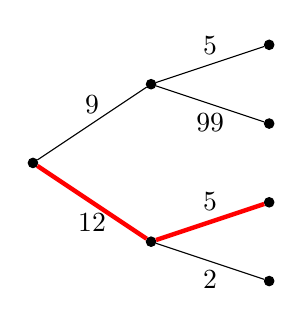
\begin{tikzpicture}

      \tikzset{enclosed/.style={draw, circle, inner sep=0pt, minimum size=.12cm, fill=black}}
% Vertices
      	\node[enclosed] (v1) at (0,2) {};
      	\node[enclosed] (v2) at (1.5,1) {};
    	\node[enclosed] (v3) at (1.5,3) {};
  	    \node[enclosed] (v4) at (3,0.5) {};
  	    \node[enclosed] (v5) at (3,1.5) {};
  	    \node[enclosed] (v6) at (3,3.5) {};
  	    \node[enclosed] (v7) at (3,2.5) {};    
%Edges
		\path (v1) edge[red, ultra thick] node[midway, below, black] {$12$} (v2);
		\path (v1) edge node[midway, above] {$9$} (v3);
		\path (v2) edge[red, ultra thick] node[midway, above, black] {$5$} (v5);
		\path (v2) edge node[midway, below] {$2$} (v4);
		\path (v3) edge node[midway, above] {$5$} (v6);
		\path (v3) edge node[midway, below] {$99$} (v7);


	\end{tikzpicture}
	\caption{Længste vej ifølge grådig algoritme.}
	\label{fig:greedy.eks}
\end{figure}

\autoref{fig:greedy.eks} et eksempel på en grådig algoritme, som har forsøgt at finde den længste mulige simple vej i en graf. Vi kan se, at algoritmen har valgt de lokalt optimale valg, men har ikke fundet den global optimale løsning. Det er tydeligt at se, at denne algoritme ikke er pålidelig nok til at løse sådanne problemer. Der findes dog nogle grådige algoritmer som er optimeret således de altid finder den globalt optimale løsning, så længe grafen overholde specifikke krav. Dette ser vi i \autoref{kap:dijkstras}


\section{Dijkstras algoritme}
I \ref{defn:min.vej} definerede vi distancen af den korteste vej i en vægtet graf. For at finde den korteste vej vil vi anvende \emph{Dijkstras algoritme}. Dijkstras algoritme kan bruges til at finde den korteste vej i en simpel, vægtet graf, hvori vægtene for alle kanter i grafen skal være ikke-negative. Algoritmen fungerer således, at den finder den korteste vej fra en startknude, $v_{1}$, til en endeknude, $v_{m}$, ved først at finde naboknuderne til $v_{1}$ og undersøge hvilken af disse, der har den mindste distanceværdi og altså er tættest på startknuden. Derefter tager den udgangspunkt i den naboknude, hvortil distanceværdien er mindst og fortsætter ad dennes vej, så længe denne vej har en mindre distanceværdi end en alternativ vej. Fremgangsmåden vil her illustreres ved hjælp af et eksempel, som tager udgangspunkt i \ref{kap:grafteori}.

\begin{exmp}
Betragt figur \ref{fig.dijkstraexmp}
\begin{figure}[H]
\centering
	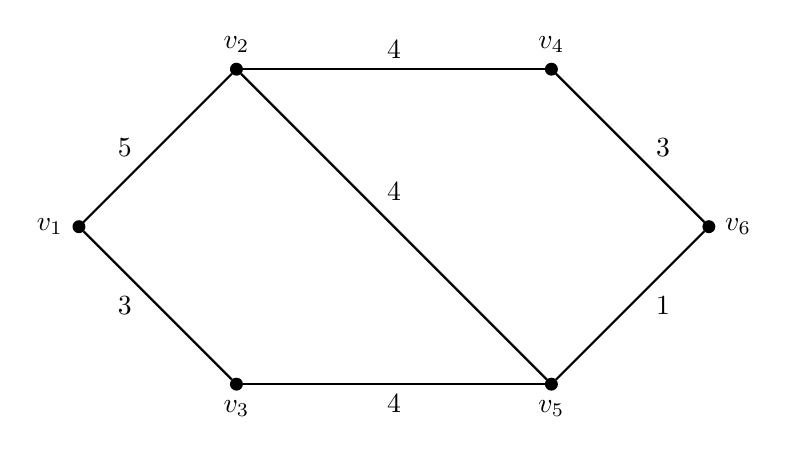
\begin{tikzpicture}

      \tikzset{enclosed/.style={draw, circle, inner sep=0pt, minimum size=.15cm, fill=black}}
%% Vertices
      	\node[enclosed, label={left: $v_1$}] (v1) at (0,2) {};
      	\node[enclosed, label={above: $v_2$}] (v2) at (2,4) {};
    	\node[enclosed, label={below: $v_3$}] (v3) at (2,0) {};
  	    \node[enclosed, label={above: $v_4$}] (v4) at (6,4) {};
     	\node[enclosed, label={below: $v_5$}] (v5) at (6,0) {};
     	\node[enclosed, label={right: $v_6$}] (v6) at (8,2) {};
%Edges
		\path [-, > = latex, thick] (v1) edge node[midway, left=2mm] {$ 5 $} (v2);
		\path [-, > = latex, thick] (v1) edge node[midway, left=2mm] {$ 3 $} (v3);
		\path [-, > = latex, thick] (v2) edge node[midway, above] {$ 4 $} (v4);
		\path [-, > = latex, thick] (v2) edge node[midway, above=2mm] {$ 4 $} (v5);
		\path [-, > = latex, thick] (v3) edge node[midway, below] {$ 4 $} (v5);
		\path [-, > = latex, thick] (v4) edge node[midway, right=2mm] {$ 3 $} (v6);
		\path [-, > = latex, thick] (v5) edge node[midway, right=2mm] {$ 1 $} (v6);

	\end{tikzpicture}
	\caption{Simpel, vægtet graf.}
	\label{fig.dijkstraexmp}
\end{figure}
I figur \ref{fig.dijkstraexmp} vil vi finde den korteste vej fra $v_{1}$ til $v_{6}$. Dijkstras algoritme vil gøre dette ved at finde den korteste vej fra startknuden, $v_{1}$, til hver knude, indtil den når endeknuden, $v_{6}$. Først vil den se, at startknuden har naboknuderne $v_{2}$ og $v_{3}$. Der er altså to veje fra startknuden, $P=(v_{1},v_{2})$ med distancen 5 og $P=(v_{1},v_{3})$ med distancen 3. Dermed er $v_{3}$ den knude, der er tættest på startknuden. Herefter er der igen to veje, $P=(v_{1},v_{2})$ med distancen 5 og $P=(v_{1},v_{3},v_{5})$ med distancen 7. Den første af disse vælges, da denne har den mindste distance, og $v_{2}$ er dermed knuden, som er næsttættest på startknuden. Nu er der tre forskellige veje, $P=(v_{1},v_{2}, v_{4})$ med distancen 9, $P=(v_{1},v_{2}, v_{5})$ med distancen 9 og $P=(v_{1},v_{3}, v_{5})$ med distancen 7. Den tredje vælges, og det er nu noteret, at den korteste vej fra $v_{1}$ til $v_{5}$ har distancen 7. Der er nu igen kun to mulige veje at vælge imellem, $P=(v_{1},v_{2}, v_{4})$ med distancen 9 og $P=(v_{1},v_{3}, v_{5}, v_{6})$ med distancen 8. $P=(v_{1},v_{2}, v_{5})$ er ikke længere en mulig vej, da vi allerede har fundet den korteste vej fra $v_{1}$ til $v_{5}$. Den anden vej har den mindste distance, og derfor vælger vi denne, og vi ved nu, at den korteste vej fra $v_{1}$ til $v_{6}$ er $P=(v_{1},v_{3}, v_{5}, v_{6})$ og har distancen 8.
\end{exmp}

Ovenstående eksempel er simpelt og kan hurtigt løses ved fx brute force metoden, men i større og mere komplicerede grafer er Dijkstras algoritme meget mere effektiv. For at skabe yderligere overblik over hvordan Dijkstras algoritme fungerer, vil vi her gå i dybden med dennes mere teoretiske del.
\begin{algorithm}[H]
\caption{Dijkstras algoritme}
\begin{algorithmic}[1]

\Procedure{dijkstra($G$: vægtet, sammenhængende, simpel graf med kun ikke-negative vægte)}{}
    \State \{$G$ {har knuderne $a = v_{1}, v_{2}, \dotsc, v_{m} = z$ og vægtene til kanterne $w(v_{i}, v_{j})$, hvor $w(v_{i}, v_{j}) = \infty$ hvis $v_{i}$ og $v_{j}$ ikke er naboer \}}
	\For {$i := 2$ \textbf{to} $m$}
		\State $L(v_{i}) := \infty$
	\EndFor
	\State $L(a) := 0$	
	\State $S := \emptyset$
	\State {\{distancen til hver knude initialiseres, så $a = 0$, og distancen til alle andre knuder er $\infty$, derudover er $S$ defineret som en tom mængde\}}
    \While{$z \notin S$}
        \State {$u :=$ en knude som ikke er i $S$ med $L(u)$ som minimum}
        \State $S := S \cup \{u\}$
        \For {alle $v \notin S$}
        	\If {$L(u) + w(u,v) < L(v)$} {$L(v) := L(u) + w(u,v)$}
        	\State \{dette tilføjer knuder til $S$ med minimal 			distance og opdaterer distancerne til
        	\State knuderne, som ikke er i $S$\}
        	\EndIf
    	\EndFor
    \EndWhile
    \State {\textbf{return} $L(z)$ \{$L(z) = \alpha(a,z)$\}} 
\EndProcedure

\end{algorithmic}
\label{alg:dijkstra}
\end{algorithm}
Det første, der sker, er, at startknuden noteres som $0$, og resten af knuderne noteres som $\infty$. Her betegnes den korteste vej som $\alpha_{k}(v_1,v_m)$, fra definition \ref{defn:min.vej}, hvor $k$ er antallet af \emph{iterationer} gennemført i algoritmen. Antallet af iterationer er det antal gange en løkke gennemkøres, altså hver gang vejen opdateres. Distancen af den korteste vej algoritmen finder fra startknuden til en given knude, noterer vi her ved $L$. $L_{0}(v_1)=0$ betyder altså, at vi har nul iterationer og dermed kun kender startknuden med distancen $0$. Derudover oprettes en mængde $S$, for hvilken det gælder, at $S = \emptyset$ når $k = 0$. Ved første iteration undersøges startknudens naboknuder, og man bestemmer, som i eksemplet ovenfor, hvilken distance er mindst. Dermed er startknudens nærmeste knude fundet, og denne tilføjes nu til mængden $S$. For hver iteration tilføjes et nyt element til mængden, og denne proces fortsætter, til algoritmen har fundet den korteste vej fra startknuden til endeknuden. Mængden, $S$, indeholder til sidst distancerne for den korteste vej fra startknuden til alle knuder i grafen. 

Ved brug af ovenstående metode kan vi illustrere løsningen til korteste vej-problemet fra \autoref{fig.dijkstraexmp} i en tabel.

\begin{table}[H]
\centering
\begin{tabular}{|c|c|c|c|c|c|c|}
\hline
$v$ & $v_1$ & $v_2$ & $v_3$ & $v_4$ & $v_5$ & $v_6$ \\ \hline
  & $\boldsymbol{0}$ &  $\infty$ & $\infty$  & $\infty$  &  $\infty$  &  $\infty$  \\  
 $v_1$ &  & $5_{v_1}$ & $\boldsymbol{3_{v_1}}$ & $\infty$ & $\infty$ & $\infty$ \\  
 $v_3$ &  & $\boldsymbol{5_{v_1}}$ &  & $\infty$ & $7_{v_3}$ & $\infty$ \\  
 $v_2$ &  &  &  & $9_{v_2}$ & $\boldsymbol{7_{v_3}}$ & $\infty$ \\
 $v_5$ &  &  &  & $9_{v_2}$ &  & $\boldsymbol{8_{v_5}}$   \\ \hline
\end{tabular}
\caption{Tabellarisk løsning til korteste vej i \autoref{fig.dijkstraexmp}.}
\label{tab:dijkstraexmp}
\end{table}

\begin{thm}[Dijkstras algoritme] \label{thm:dijkstra}
Dijkstras algoritme finder distancen af den korteste vej mellem to knuder, $v_1,v_m$, i en vægtet, sammenhængende og simpel graf sådan at $L(v_m)=\alpha(v_1,v_m)$. 
\end{thm}

\begin{proof}
Sætning \ref{thm:dijkstra} kan bevises ved induktion. Ved et induktionsbevis etablerer vi først et basisskridt, og dernæst opstiller vi en induktionshypotese. Basisskridtet består blot i, at vi undersøger distancen fra startknuden til startknuden, som selvfølgelig er 0, hvilket algoritmen også noterer. Vi har dermed $L(v_1)=0= \alpha(v_1,v_1)$, hvilket er sandt.
Vi opstiller nu vores induktionshypotese, hvor vi antager, at Sætning \ref{thm:dijkstra} er sand for $k$ iterationer. Det gælder altså at

\begin{equation}
L(v_m) = \alpha(v_1,v_m), \forall v \in S_k \textrm{ for vejen } P = (v_1, v_2, \dotsc, v_m).
\end{equation}
Vi sætter nu $v_{n}$ til at være den knude, der tilføjes til $S$ ved $S_{k+1}$. Vi vil nu vise, at det ligesom ved alle tidligere knuder i $S$ også gælder for $v_{n}$ at $L(v_n)=\alpha(v_1,v_n)$. Dette kan bevises ved modstrid. Vi starter med at antage, at der findes en kortere vej fra $v_1$ til $v_n$ end $L(v_n)$. Vi kalder denne nye vej $P_1$. For denne må det gælde at

\begin{equation}
dist(P_1)<L(v_n).
\end{equation}
$P_1$ starter i $S_k$ og forlader på et tidspunkt denne mængde for at komme til $v_n$, som ikke er i $S_k$. Vi lader $v_x,v_y$ være den første kant på vejen $P_1$, der forlader $S_k$. $P_x$ betegnes som delen af vejen $P_1$, som går fra $v_1$ til $v_x$. Så ved vi at

\begin{equation}
dist(P_x)+w(v_x,v_y) \leq dist(P_1).
\end{equation}
Eftersom $v_x$ er i $S_k$, ved vi som følge af induktionshypotesen, at den korteste vej fra $v_1$ til $v_x$ er $L(v_x)$. Dermed ved vi at $L(v_x) \leq dist(P_x)$ og

\begin{equation}
L(v_x) + w(v_x,v_y) \leq dist(P_1).
\end{equation}
$v_y$ er nabo til $v_x$, hvilket betyder at

\begin{equation}
L(v_y) \leq L(v_x) + w(v_x,v_y).
\end{equation}
Eftersom hverken $v_n$ eller $v_y$ er i $S_k$, og algoritmen oprindeligt valgte $v_n$ i den $k+1$'te iteration, må $v_n$ have den mindste distance af de to således at

\begin{equation}
L(v_n) \leq L(v_y).
\end{equation}
Dette resulterer dog i, at vi påstår, at $L(v_n) < L(v_n)$. Dette kan ikke lade sig gøre, og vi konkluderer derfor, at der ikke findes en tilfældig kortere vej, $P_1$. $L(v_n)=\alpha(v_1,v_n)$ må altså være sandt, og Dijkstra algoritme finder den korteste vej.
\end{proof}

\section{Kompleksitet} \label{kap:kompleksitet}
%side 250 ish
%table 1 side 247 i pdf.

Der findes to former for kompleksitet, men vi vælger at fokusere på tidskompleksitet. Den anden form for kompleksitet er pladskompleksitet. 
Der er tre former for tilfælde: bedste, værste og gennemsnitlige. 
I bedste tilfælde ser man på det laveste antal trin for en inputstørrelse, $n$. I værste ser man på det højeste og i gennemsnittet, det gennemsnitlige. 
\emph{Bedste tilfælde} beskriver algoritmen under optimale forhold, i en lineær søgealgoritme vil dette altså være, at elementet der søges efter, er det første element i listen. 
Oftere ser man på enten \emph{værste tilfælde} eller \emph{gennemsnitlige tilfælde}. 
Det gennemsnitlige tilfælde vil give et rigtigt godt overblik over hvor god algoritmen er, dog er det meget svært at bestemme hvad et gennemsnitligt input er, da det er svært at bestemme nogle parametre at vælge ud fra. 
Det værste tilfælde giver et godt overblik over hvor lang tid det kan tage. Ved man at algoritmen er lineær i værste tilfælde, vil man kunne løse den i rimelig tid for alle størrelser $n$.
De forskellige resultater i vores analyse af algoritmerne, kan deles op i kategorier, de mest gængse er: $\log n$, $\sqrt{n}$, $n$, $n^x$, $x^n$ og $n!$, men det kan også være en kombination af disse, som $n!n$, $n\log n$ eller lignende.
For at beskrive disse algoritmer i fx værste tilfælde, vil man bruge operatorerne \emph{store-O}, \emph{store-Omega} og \emph{Theta}. Man vil her fokusere på \emph{asymptotiske $n$-værdier}, altså ved rigtigt store værdier for $n$, da man i nogle tilfælde vil have en algoritme der er langsommere end den øvre bindende funktion ved små $n$, men ved større, som fx over 10.000, er hurtigere.

\subsection{Store-$O$}
\begin{defn}
$f(n)= O(g(n))$ hvis og kun hvis $\exists$ positive konstanter $C$ og $n_o$ så at $|f(n)| \leq C |g(n)| \forall n \geq n_o$.
\end{defn}

Store-$O$ bliver brugt til at binde funktionen opadtil, begrænse den oppe fra. Man kan med garanti sige, at algoritmen tager store-$O$ tid eller mindre. 
\begin{exmp}
\begin{align*}
f(n)=& 13n+3 \\
13n+3 \leq& 20n \forall \ n \geq 1 \\
f(n) =& O(n).
\end{align*}
\end{exmp}
Man vil også kunne sige, at $f(n)$ er mindre end $n!$ eller en anden vilkårlig højere funktion $g(n)$, men da man altid vil vælge den mest begrænsende funktion, vil $n$ være det mest præcise. 

\subsection{Store-$\Omega$}
\begin{defn}
$f(n) = \Omega(g(n))$ hvis og kun hvis $\exists$ positive konstanter $C$ og $n_o$ så at $|f(n)| \geq C |g(n)| \forall n \geq n_o$.
\end{defn}
Store-Omega bruges, omvendt store-$O$, til at binde funktionen nedadtil, altså finde den nedre grænse for algoritmen, den vil mindst tage store-Omega tid i det givne tilfælde.
\begin{exmp}
\begin{align*}
f(n)=& 13n+3 \\
13n+3 \geq& n \forall \ n \geq 1 \\
f(n) =& \Omega(n).
\end{align*}
\end{exmp}

På samme måde som ved store-$O$-notationen, vil man her kunne vælge en vilkårlig mindre funktion, $logn$, $1$ med flere, men da man vil begrænse den så meget som muligt, vælger man den største funktion $g(n)$ hvor uligheden stadig er sand.
\subsection{Store-$\Theta$}
\begin{defn}
$f(n) = \Theta(g(x))$ hvis og kun hvis $\exists$ positive konstanter $C_1, C_2$ og $n_o$ så at $C_1|g(n)| \leq |f(n)| \leq C_2|g(n)| \forall n \geq n_o$.
\end{defn}
Når man har fundet den øvre og den nedre grænse, store-O og store-Omega, kan man finde Theta, den tætte bundne funktion,
\begin{exmp}
\begin{align*}
f(n)=& 13n+3 \\
\Omega(n) \leq& f(n) \leq O(n) \\
n \leq& 13n+3 \leq 10n \forall \ n \geq 1 \\
f(n) =& \Theta(n).
\end{align*}
\end{exmp}

I følgende afsnit tager vi udgangspunkt i to sorteringer, og ser hvordan de sammenligner sig på Store-$O$ i bedste og værste tilfælde.

\subsection{Kompleksitet af bubblesortering} \label{kap:kom_bubble}

For at finde kompleksiteten af bubblesortering, bruger vi store-$O$-notationen fra tidligere. 
Bubblesortering, som nævnt i \autoref{kap:sortering}, sammenligner to elementer fra listen, og flytter rundt på dem, hvis de står i forkert rækkefølge.
Vi starter med værste tilfælde. Her ser vi på en liste, $P$, der er sorteret i omvendt rækkefølge. $P = (5,4,3,2,1)$.
i første gennemgang sammenligner den 5 med 4, og bytter om, 5 med 3, bytter igen, 5 med 2, bytter, og til sidst 5 med 1, nu står 5 korrekt og $P = (4, 3, 2, 1, 5)$
Efter næste gennemgang er $P = (3, 2, 1, 4, 5)$ og de sidste gennemgange medfører hhv. $(2, 1, 3, 4, 5)$ og $(1, 2, 3, 4, 5)$. Her ses altså, at der gennemføres 5 gennemgange, eller $n$ gange. 
For hver gang den sammenligner, gør den det $n-1$ gange. 
Derved er kompleksiteten $O(n\times n)$ eller $O(n^2)$.

I bedste tilfælde er listen, $P$, lig $(1, 2, 3, 4, 5)$.
Her ses altså at der kun gennemføres én gennemgang, og der stadig udføres $n-1$ sammenligninger i denne gennemgang.
Som vi kender fra tidligere teori, tælles de mindre ordner ikke med, derved er kompleksiteten $O(1n)$, eller $O(n)$. 

\subsection{Kompleksitet af indskudssortering} \label{kap:kom_indskud}
En anden sorteringsalgoritme fra \autoref{kap:sortering} er indskudssorteringen. 
Denne tager udgangspunkt i et enkelt input af gangen og sammenligner dette med resten af den sorterede liste.
Hvis vi igen benytter det værste tilfælde, $P = (5,4,3,2,1)$, ser vi at den først tager femtallen, og sætter ind i listen, herefter sammenligner den næste element i $P$ med den sorterede liste, der kun indeholder 5, dermed er den sorterede liste $Q = (5,4)$ og $P=(3,2,1)$. 
Herefter indsættes 3 i listen $Q$ og sammenlignes først med 5, og herefter 4, hvorefter det indsættes før de to, så listen er $Q = (3,4,5)$, på samme måde indsættes de sidste to input i listen $Q$ og dermed er den fuldført.
Vi ser her at der, på samme måde som med bubblesortering, køres 5 gennemgange. Der er i første gennemgang 0 sammenlininger, derefter 1 sammenligning i anden gennemgang og $m-1$ sammenligninger i $n$'de gennemgang. Hermed er denne sortering også $O(n^2)$ i værste fald.

I bedste fald, når $P= (1,2,3,4,5)$ har den en lineær kompleksitet, da den, i alle gennemgange, kun sammenlininger med det element der er længst til højre hvorefter det er indsat korrekt, dermed er kompleksiteten $O(n)$.



P \\
NP \\
NP-Complete \\
NP-Hard. 



%\pgfplotsset{compat=1.10}
%\usepgfplotslibrary{fillbetween}

%\begin{figure}[H]
%\centering
%	\begin{tikzpicture}
%\begin{axis}[
%    xmin=0, xmax=10,
%    ymin=0, ymax=10
%    ]

%    \addplot [name path=plot1, ultra thin, domain=-10:10, samples=150]{x^2};
%    \addplot [name path=plot2, ultra thin, domain=-10:10, samples=150]{2*x+4};


%\end{axis}
%	\end{tikzpicture}
%	\caption{Kompleksitet}
%	\label{fig.kompleksitet}
%\end{figure}
\section{NP-problemer} \label{kap:np}
Problemer kan alt efter deres tidskompleksitet inddeles i forskellige kategorier. Hvis et problem kan løses i polynomisk tid af en \emph{deterministisk} algoritme, kaldes problemet \emph{P}, som står for polynomial time.
At en algoritme er deterministisk, betyder, at man kender alle trin i algorimen, og at den ikke indeholder nogle tilfældige hændelser. Vi så i \autoref{kap:kompleksitet} nogle eksempler på algoritmer med polynomisk kompleksitet. Vi ved fx, at den lineære søgning, den binære søgning, bubblesortering og indskudssortering er deterministiske algoritmer, som løser problemer i polynomisk tid og dermed løser P problemer. 
Et problem løst med en \emph{ikke-deterministisk} algoritme, i polynomisk tid, kaldes \emph{NP}, hvilket står for Non-deterministic Polynomial time. En ikke-deterministisk algoritme indeholder, i modsætning til den deterministiske, tilfældige hændelser, som kan have kendte sandsynligheder. Her kender vi ikke alle trin, algoritmen skal gennemføre. 

Et NP problem kan med tiden blive et P problem, hvis vi finder en deterministisk algoritme, der kan løse dette i polynomisk tid. P er desuden en delmængde af NP, da P problemer også kan løses af en ikke-deterministisk algoritme i polynomisk tid, men P adskiller sig ved at være de problemer i NP, som også kan løses af en deterministisk algoritme. 
Der er stor debat om hvorvidt, alle problemer i NP kan løses med en deterministisk algoritme. Problemer, vi troede var NP for nogle år siden, kan nu løses med en deterministisk algoritme. Det er dog stadig uklart, om dette er gældende for alle NP problemer.


%------------------------------------------ rettet opad herfra.
Problemer kan derudover være \emph{NP-complete} og \emph{NP-hard}. Et problem er NP-complete, hvis alle NP problemer kan reduceres til dette problem, og hvis problemet selv er et NP problem. Løsningen skal altså kunne verificeres i polynomisk tid, da dette gælder for NP problemer. Hvis man har et NP-complete problem B, som kan reduceres til et problem A i polynomisk tid, hvor A også kan løses i polynomisk tid af en ikke-deterministisk algoritme, vil A desuden også være et NP-complete problem. Der findes mange NP-complete problemer, men det er endnu ikke lykkedes at løse nogen af dem med en deterministisk algoritme i polynomisk tid.

Et problem er NP-hard, hvis alle NP problemer kan reduceres til dette problem, og hvis løsningen ikke kan verificeres i polynomisk tid. Det er altså meget vanskeligt at vise, om et problem er NP-hard. Et NP-hard problem er mindst lige så svært som det sværeste problem i NP. Dette skyldes, at alle NP problemer skal kunne reduceres til et vilkårligt NP-hard problem.
De forskellige problemtyper ses illustreret herunder:




\begin{figure}[H]
\centering
	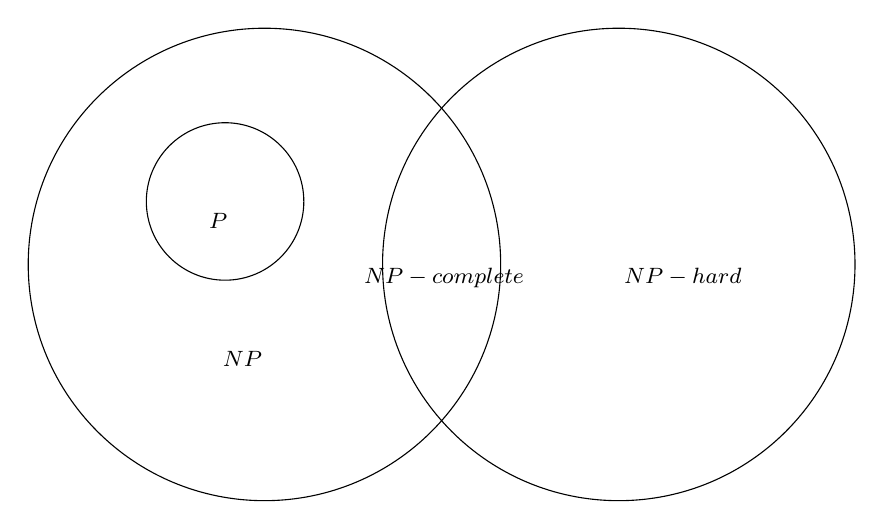
\begin{tikzpicture}
      \draw (0,2) circle (3cm);
      \put(-15,20){{\footnotesize $NP$}};
      \draw (4.5,2) circle (3cm);
      \put(130,50){{\footnotesize $NP-hard$}};
      \draw (-0.5,2.8) circle (1cm);
      \put(-20,70){{\footnotesize $P$}};
      \put(36,50){{\footnotesize $NP-complete$}};
	\end{tikzpicture}
	\caption{P, NP, NP-hard og NP-complete.}
	\label{fig.dijkstraexmp}
\end{figure}

Hvis vi kigger på Dijkstras algoritme i \autoref{kap:dijkstras}, ser vi, at denne algoritme løser problemer af typen P. Problemerne løses af en deterministisk algoritme i polynomisk tid, da grafen i et korteste vej-problem har optimal substruktur.

Dijkstras algoritme løser korteste vej-problemer, men ønsker vi at finde den længste vej igennem en orienteret ikke-cyklisk graf, er dette også et P problem. Havde grafen fx været ikke-orienteret og cyklisk, havde det været et NP-complete problem, men beviset udelades. Vigtigt at notere er blot, at disse ikke kan løses af en deterministisk algoritme, da grafen i disse længste vej-problemer ikke har optimal substruktur.
I Eksempel \ref{exmp.np} ses det, hvordan substrukturen i en ikke-orienteret, cyklisk graf er, for henholdsvis korteste og længste vej-problemer.

\begin{exmp} \label{exmp.np}
På \autoref{fig:laengste.vej} ses det, at den korteste vej  fra $v_1$ til $v_4$ går igennem punktet $v_2$. Den korteste vej har optimal substruktur, hvilket ses ved, at den korteste vej fra $v_{1}$ til $v_{4}$, $P_{1,2,4}=(v_{1},v_{2},v_{4})$, består af den korteste vej fra $v_{1}$ til $v_{2}$ og den korteste vej fra $v_{2}$ til $v_{4}$. 

Vi ser nu på den længste vej fra $v_1$ til $v_4$, $P_{1,2,4}=(v_{1},v_{2},v_{4})$ Hvis der havde været optimal substruktur, havde den længste vej, $P_{1,2,4}$, bestået af den længste vej fra $v_{1}$ til $v_{2}$ og den længste vej fra $v_{2}$ til $v_{4}$, men dette er ikke tilfældet. Den længste vej igennem grafen fra $v_{1}$ til $v_{2}$ er nemlig $P_{1,3,4,2}=(v_{1},v_{3},v_{4},v_{2})$, og den længste vej igennem grafen fra $v_{2}$ til $v_{4}$ er $P_{2,1,3,4}=(v_{2},v_{1},v_{3},v_{4})$. 




\begin{figure}[H]
\centering
	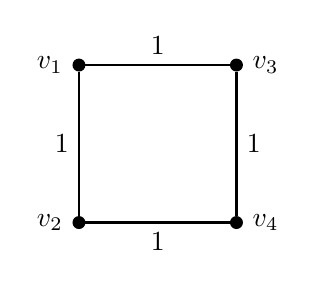
\begin{tikzpicture}
      \tikzset{enclosed/.style={draw, circle, inner sep=0pt, minimum size=.15cm, fill=black}}
%% Vertices
	%ikke orienteret
      	\node[enclosed, label={left, above: $v_1$}] (v1) at (0,2) {};
     	\node[enclosed, label={left, below: $v_2$}] (v2) at (0,0) {};
     	\node[enclosed, label={right, above: $v_3$}] (v3) at (2,2) {};
     	\node[enclosed, label={right, below: $v_4$}] (v4) at (2,0) {};    	
%Edges
	%Ikke orientered
		\path [thick] (v1) edge node[midway, left] {1} (v2);
		\path [thick] (v1) edge node[midway, above] {1} (v3);
		\path [thick] (v2) edge node[midway, below] {1} (v4);
		\path [thick] (v3) edge node[midway, right] {1} (v4);

\end{tikzpicture}
	\caption{Simpel vægtet graf.}
	\label{fig:laengste.vej}
\end{figure}

\end{exmp}


